% \documentclass{article}
\documentclass[12pt,a4paper,oneside,fleqn]{book}
\usepackage[slovene]{babel}
% \usepackage[english]{babel}

% \usepackage[a4paper,top=2cm,bottom=2cm,left=3cm,right=3cm,marginparwidth=1.75cm]{geometry}
\usepackage[left=30mm,
right=25mm,
top=30mm,
bottom=25mm]{geometry}

% \usepackage[backend=biber, style=ieee]{biblatex}
\usepackage{cite}
\usepackage[numbib]{tocbibind}
% \addbibresource{refs.bib}

\usepackage{lipsum}
\usepackage{array}
\usepackage{caption}
\usepackage{amsmath}
\usepackage{graphicx}
\usepackage{subcaption}
\usepackage[colorlinks=true, allcolors=blue]{hyperref}
\usepackage[nodisplayskipstretch]{setspace}
\usepackage{fancyhdr}
\usepackage{listings}
\usepackage{xcolor}
\usepackage{float}

\definecolor{codegreen}{rgb}{0,0.6,0}
\definecolor{codegray}{rgb}{0.5,0.5,0.5}
\definecolor{codepurple}{rgb}{0.58,0,0.82}
\definecolor{backcolour}{rgb}{0.95,0.95,0.92}

\lstdefinestyle{codestyle}{
    backgroundcolor=\color{backcolour},   
    commentstyle=\color{codegreen},
    keywordstyle=\color{magenta},
    numberstyle=\tiny\color{codegray},
    stringstyle=\color{codepurple},
    basicstyle=\ttfamily\footnotesize,
    breakatwhitespace=false,         
    breaklines=true,                 
    captionpos=b,                    
    keepspaces=true,                 
    % numbers=left,   
    numbers=none,
    numbersep=5pt,                  
    showspaces=false,                
    showstringspaces=false,
    showtabs=false,                  
    tabsize=2
}
\renewcommand{\lstlistingname}{Kod}
\lstset{style=codestyle}


%paragraph settings
\setlength\parindent{0pt}
\setlength{\parskip}{1.5ex plus 0.5ex minus 0.5ex}

% set equation environment indentation
\setlength{\mathindent}{0.5cm}%

% set itemize environment whitespacing and left margin
% \setlist[itemize]{noitemsep,nolistsep, leftmargin=*}

% set table and figure captions
\captionsetup[table]{skip=10pt,singlelinecheck=false}
\captionsetup[figure]{justification=centering}

% set tablename to Preglednica
\AtBeginDocument{%
	\renewcommand\tablename{Preglednica}
}

% set section and tableofcontents depth
\setcounter{secnumdepth}{3}
\setcounter{tocdepth}{3}
\def\labelitemi{--}

%  accordingly format a chapter definition
% \titleformat{\chapter}[display]
% {\bfseries}{}{0pt}{\Huge\thechapter\quad}

% set fancy_nohead fancy header
\fancypagestyle{fancy_nohead}{
	\fancyfoot[RO]{\thepage}
	\fancyhead{}
	\renewcommand{\headrulewidth}{0pt}
	\chead{}
	\cfoot{}
}

% assign no_header
% \assignpagestyle{\chapter}{fancy_nohead}

\renewcommand{\thetable}{\arabic{chapter}.\arabic{table}}
\renewcommand{\thefigure}{\arabic{chapter}.\arabic{figure}}
\renewcommand{\theequation}{\arabic{chapter}.\arabic{equation}}

% \renewcommand\cftchapdotsep{\cftdotsep}  % adds leader dots from chapter titles to page numbers

\usepackage[T1]{fontenc} % Ensures proper font rendering
\usepackage{lmodern}  
\usepackage[mmyyyy]{datetime}
% \newdateformat{mydate}{\shortmonthname[\THEMONTH], \THEYEAR}
 %%%%%%%%%%%%%%%%%%%%%%%%%%%%%%%%%%%%%%%%%%%%%%%%%%%%%%%%%%%%%%%%%%%%%%%%%%%%%%%% 
%%% ~ Arduino Language - Arduino IDE Colors ~                                  %%%
%%%                                                                            %%%
%%% Kyle Rocha-Brownell | 10/2/2017 | No Licence                               %%%
%%% -------------------------------------------------------------------------- %%%
%%%                                                                            %%%
%%% Place this file in your working directory (next to the latex file you're   %%%
%%% working on).  To add it to your project, place:                            %%%
%%%     %%%%%%%%%%%%%%%%%%%%%%%%%%%%%%%%%%%%%%%%%%%%%%%%%%%%%%%%%%%%%%%%%%%%%%%%%%%%%%%% 
%%% ~ Arduino Language - Arduino IDE Colors ~                                  %%%
%%%                                                                            %%%
%%% Kyle Rocha-Brownell | 10/2/2017 | No Licence                               %%%
%%% -------------------------------------------------------------------------- %%%
%%%                                                                            %%%
%%% Place this file in your working directory (next to the latex file you're   %%%
%%% working on).  To add it to your project, place:                            %%%
%%%     %%%%%%%%%%%%%%%%%%%%%%%%%%%%%%%%%%%%%%%%%%%%%%%%%%%%%%%%%%%%%%%%%%%%%%%%%%%%%%%% 
%%% ~ Arduino Language - Arduino IDE Colors ~                                  %%%
%%%                                                                            %%%
%%% Kyle Rocha-Brownell | 10/2/2017 | No Licence                               %%%
%%% -------------------------------------------------------------------------- %%%
%%%                                                                            %%%
%%% Place this file in your working directory (next to the latex file you're   %%%
%%% working on).  To add it to your project, place:                            %%%
%%%    \input{arduinoLanguage.tex}                                             %%%
%%% somewhere before \begin{document} in your latex file.                      %%%
%%%                                                                            %%%
%%% In your document, place your arduino code between:                         %%%
%%%   \begin{lstlisting}[language=Arduino]                                     %%%
%%% and:                                                                       %%%
%%%   \end{lstlisting}                                                         %%%
%%%                                                                            %%%
%%% Or create your own style to add non-built-in functions and variables.      %%%
%%%                                                                            %%%
 %%%%%%%%%%%%%%%%%%%%%%%%%%%%%%%%%%%%%%%%%%%%%%%%%%%%%%%%%%%%%%%%%%%%%%%%%%%%%%%% 

\usepackage{color}
\usepackage{listings}    
\usepackage{courier}

%%% Define Custom IDE Colors %%%
\definecolor{arduinoGreen}    {rgb} {0.17, 0.43, 0.01}
\definecolor{arduinoGrey}     {rgb} {0.47, 0.47, 0.33}
\definecolor{arduinoOrange}   {rgb} {0.8 , 0.4 , 0   }
\definecolor{arduinoBlue}     {rgb} {0.01, 0.61, 0.98}
\definecolor{arduinoDarkBlue} {rgb} {0.0 , 0.2 , 0.5 }

%%% Define Arduino Language %%%
\lstdefinelanguage{Arduino}{
  language=C++, % begin with default C++ settings 
%
%
  %%% Keyword Color Group 1 %%%  (called KEYWORD3 by arduino)
  keywordstyle=\color{arduinoGreen},   
  deletekeywords={  % remove all arduino keywords that might be in c++
                break, case, override, final, continue, default, do, else, for, 
                if, return, goto, switch, throw, try, while, setup, loop, export, 
                not, or, and, xor, include, define, elif, else, error, if, ifdef, 
                ifndef, pragma, warning,
                HIGH, LOW, INPUT, INPUT_PULLUP, OUTPUT, DEC, BIN, HEX, OCT, PI, 
                HALF_PI, TWO_PI, LSBFIRST, MSBFIRST, CHANGE, FALLING, RISING, 
                DEFAULT, EXTERNAL, INTERNAL, INTERNAL1V1, INTERNAL2V56, LED_BUILTIN, 
                LED_BUILTIN_RX, LED_BUILTIN_TX, DIGITAL_MESSAGE, FIRMATA_STRING, 
                ANALOG_MESSAGE, REPORT_DIGITAL, REPORT_ANALOG, SET_PIN_MODE, 
                SYSTEM_RESET, SYSEX_START, auto, int8_t, int16_t, int32_t, int64_t, 
                uint8_t, uint16_t, uint32_t, uint64_t, char16_t, char32_t, operator, 
                enum, delete, bool, boolean, byte, char, const, false, float, double, 
                null, NULL, int, long, new, private, protected, public, short, 
                signed, static, volatile, String, void, true, unsigned, word, array, 
                sizeof, dynamic_cast, typedef, const_cast, struct, static_cast, union, 
                friend, extern, class, reinterpret_cast, register, explicit, inline, 
                _Bool, complex, _Complex, _Imaginary, atomic_bool, atomic_char, 
                atomic_schar, atomic_uchar, atomic_short, atomic_ushort, atomic_int, 
                atomic_uint, atomic_long, atomic_ulong, atomic_llong, atomic_ullong, 
                virtual, PROGMEM,
                Serial, Serial1, Serial2, Serial3, SerialUSB, Keyboard, Mouse,
                abs, acos, asin, atan, atan2, ceil, constrain, cos, degrees, exp, 
                floor, log, map, max, min, radians, random, randomSeed, round, sin, 
                sq, sqrt, tan, pow, bitRead, bitWrite, bitSet, bitClear, bit, 
                highByte, lowByte, analogReference, analogRead, 
                analogReadResolution, analogWrite, analogWriteResolution, 
                attachInterrupt, detachInterrupt, digitalPinToInterrupt, delay, 
                delayMicroseconds, digitalWrite, digitalRead, interrupts, millis, 
                micros, noInterrupts, noTone, pinMode, pulseIn, pulseInLong, shiftIn, 
                shiftOut, tone, yield, Stream, begin, end, peek, read, print, 
                println, available, availableForWrite, flush, setTimeout, find, 
                findUntil, parseInt, parseFloat, readBytes, readBytesUntil, readString, 
                readStringUntil, trim, toUpperCase, toLowerCase, charAt, compareTo, 
                concat, endsWith, startsWith, equals, equalsIgnoreCase, getBytes, 
                indexOf, lastIndexOf, length, replace, setCharAt, substring, 
                toCharArray, toInt, press, release, releaseAll, accept, click, move, 
                isPressed, isAlphaNumeric, isAlpha, isAscii, isWhitespace, isControl, 
                isDigit, isGraph, isLowerCase, isPrintable, isPunct, isSpace, 
                isUpperCase, isHexadecimalDigit, 
                }, 
  morekeywords={   % add arduino structures to group 1
                break, case, override, final, continue, default, do, else, for, 
                if, return, goto, switch, throw, try, while, setup, loop, export, 
                not, or, and, xor, include, define, elif, else, error, if, ifdef, 
                ifndef, pragma, warning,
                }, 
% 
%
  %%% Keyword Color Group 2 %%%  (called LITERAL1 by arduino)
  keywordstyle=[2]\color{arduinoBlue},   
  keywords=[2]{   % add variables and dataTypes as 2nd group  
                HIGH, LOW, INPUT, INPUT_PULLUP, OUTPUT, DEC, BIN, HEX, OCT, PI, 
                HALF_PI, TWO_PI, LSBFIRST, MSBFIRST, CHANGE, FALLING, RISING, 
                DEFAULT, EXTERNAL, INTERNAL, INTERNAL1V1, INTERNAL2V56, LED_BUILTIN, 
                LED_BUILTIN_RX, LED_BUILTIN_TX, DIGITAL_MESSAGE, FIRMATA_STRING, 
                ANALOG_MESSAGE, REPORT_DIGITAL, REPORT_ANALOG, SET_PIN_MODE, 
                SYSTEM_RESET, SYSEX_START, auto, int8_t, int16_t, int32_t, int64_t, 
                uint8_t, uint16_t, uint32_t, uint64_t, char16_t, char32_t, operator, 
                enum, delete, bool, boolean, byte, char, const, false, float, double, 
                null, NULL, int, long, new, private, protected, public, short, 
                signed, static, volatile, String, void, true, unsigned, word, array, 
                sizeof, dynamic_cast, typedef, const_cast, struct, static_cast, union, 
                friend, extern, class, reinterpret_cast, register, explicit, inline, 
                _Bool, complex, _Complex, _Imaginary, atomic_bool, atomic_char, 
                atomic_schar, atomic_uchar, atomic_short, atomic_ushort, atomic_int, 
                atomic_uint, atomic_long, atomic_ulong, atomic_llong, atomic_ullong, 
                virtual, PROGMEM,
                },  
% 
%
  %%% Keyword Color Group 3 %%%  (called KEYWORD1 by arduino)
  keywordstyle=[3]\bfseries\color{arduinoOrange},
  keywords=[3]{  % add built-in functions as a 3rd group
                Serial, Serial1, Serial2, Serial3, SerialUSB, Keyboard, Mouse,
                },      
%
%
  %%% Keyword Color Group 4 %%%  (called KEYWORD2 by arduino)
  keywordstyle=[4]\color{arduinoOrange},
  keywords=[4]{  % add more built-in functions as a 4th group
                abs, acos, asin, atan, atan2, ceil, constrain, cos, degrees, exp, 
                floor, log, map, max, min, radians, random, randomSeed, round, sin, 
                sq, sqrt, tan, pow, bitRead, bitWrite, bitSet, bitClear, bit, 
                highByte, lowByte, analogReference, analogRead, 
                analogReadResolution, analogWrite, analogWriteResolution, 
                attachInterrupt, detachInterrupt, digitalPinToInterrupt, delay, 
                delayMicroseconds, digitalWrite, digitalRead, interrupts, millis, 
                micros, noInterrupts, noTone, pinMode, pulseIn, pulseInLong, shiftIn, 
                shiftOut, tone, yield, Stream, begin, end, peek, read, print, 
                println, available, availableForWrite, flush, setTimeout, find, 
                findUntil, parseInt, parseFloat, readBytes, readBytesUntil, readString, 
                readStringUntil, trim, toUpperCase, toLowerCase, charAt, compareTo, 
                concat, endsWith, startsWith, equals, equalsIgnoreCase, getBytes, 
                indexOf, lastIndexOf, length, replace, setCharAt, substring, 
                toCharArray, toInt, press, release, releaseAll, accept, click, move, 
                isPressed, isAlphaNumeric, isAlpha, isAscii, isWhitespace, isControl, 
                isDigit, isGraph, isLowerCase, isPrintable, isPunct, isSpace, 
                isUpperCase, isHexadecimalDigit, 
                },      
%
%
  %%% Set Other Colors %%%
  stringstyle=\color{arduinoDarkBlue},    
  commentstyle=\color{arduinoGrey},    
%          
%   
  %%%% Line Numbering %%%%
  numbers=left,                    
  numbersep=5pt,                   
  numberstyle=\color{arduinoGrey},    
  %stepnumber=2,                      % show every 2 line numbers
%
%
  %%%% Code Box Style %%%%
  breaklines=true,                    % wordwrapping
  tabsize=2,         
  basicstyle=\ttfamily  
}
                                             %%%
%%% somewhere before \begin{document} in your latex file.                      %%%
%%%                                                                            %%%
%%% In your document, place your arduino code between:                         %%%
%%%   \begin{lstlisting}[language=Arduino]                                     %%%
%%% and:                                                                       %%%
%%%   \end{lstlisting}                                                         %%%
%%%                                                                            %%%
%%% Or create your own style to add non-built-in functions and variables.      %%%
%%%                                                                            %%%
 %%%%%%%%%%%%%%%%%%%%%%%%%%%%%%%%%%%%%%%%%%%%%%%%%%%%%%%%%%%%%%%%%%%%%%%%%%%%%%%% 

\usepackage{color}
\usepackage{listings}    
\usepackage{courier}

%%% Define Custom IDE Colors %%%
\definecolor{arduinoGreen}    {rgb} {0.17, 0.43, 0.01}
\definecolor{arduinoGrey}     {rgb} {0.47, 0.47, 0.33}
\definecolor{arduinoOrange}   {rgb} {0.8 , 0.4 , 0   }
\definecolor{arduinoBlue}     {rgb} {0.01, 0.61, 0.98}
\definecolor{arduinoDarkBlue} {rgb} {0.0 , 0.2 , 0.5 }

%%% Define Arduino Language %%%
\lstdefinelanguage{Arduino}{
  language=C++, % begin with default C++ settings 
%
%
  %%% Keyword Color Group 1 %%%  (called KEYWORD3 by arduino)
  keywordstyle=\color{arduinoGreen},   
  deletekeywords={  % remove all arduino keywords that might be in c++
                break, case, override, final, continue, default, do, else, for, 
                if, return, goto, switch, throw, try, while, setup, loop, export, 
                not, or, and, xor, include, define, elif, else, error, if, ifdef, 
                ifndef, pragma, warning,
                HIGH, LOW, INPUT, INPUT_PULLUP, OUTPUT, DEC, BIN, HEX, OCT, PI, 
                HALF_PI, TWO_PI, LSBFIRST, MSBFIRST, CHANGE, FALLING, RISING, 
                DEFAULT, EXTERNAL, INTERNAL, INTERNAL1V1, INTERNAL2V56, LED_BUILTIN, 
                LED_BUILTIN_RX, LED_BUILTIN_TX, DIGITAL_MESSAGE, FIRMATA_STRING, 
                ANALOG_MESSAGE, REPORT_DIGITAL, REPORT_ANALOG, SET_PIN_MODE, 
                SYSTEM_RESET, SYSEX_START, auto, int8_t, int16_t, int32_t, int64_t, 
                uint8_t, uint16_t, uint32_t, uint64_t, char16_t, char32_t, operator, 
                enum, delete, bool, boolean, byte, char, const, false, float, double, 
                null, NULL, int, long, new, private, protected, public, short, 
                signed, static, volatile, String, void, true, unsigned, word, array, 
                sizeof, dynamic_cast, typedef, const_cast, struct, static_cast, union, 
                friend, extern, class, reinterpret_cast, register, explicit, inline, 
                _Bool, complex, _Complex, _Imaginary, atomic_bool, atomic_char, 
                atomic_schar, atomic_uchar, atomic_short, atomic_ushort, atomic_int, 
                atomic_uint, atomic_long, atomic_ulong, atomic_llong, atomic_ullong, 
                virtual, PROGMEM,
                Serial, Serial1, Serial2, Serial3, SerialUSB, Keyboard, Mouse,
                abs, acos, asin, atan, atan2, ceil, constrain, cos, degrees, exp, 
                floor, log, map, max, min, radians, random, randomSeed, round, sin, 
                sq, sqrt, tan, pow, bitRead, bitWrite, bitSet, bitClear, bit, 
                highByte, lowByte, analogReference, analogRead, 
                analogReadResolution, analogWrite, analogWriteResolution, 
                attachInterrupt, detachInterrupt, digitalPinToInterrupt, delay, 
                delayMicroseconds, digitalWrite, digitalRead, interrupts, millis, 
                micros, noInterrupts, noTone, pinMode, pulseIn, pulseInLong, shiftIn, 
                shiftOut, tone, yield, Stream, begin, end, peek, read, print, 
                println, available, availableForWrite, flush, setTimeout, find, 
                findUntil, parseInt, parseFloat, readBytes, readBytesUntil, readString, 
                readStringUntil, trim, toUpperCase, toLowerCase, charAt, compareTo, 
                concat, endsWith, startsWith, equals, equalsIgnoreCase, getBytes, 
                indexOf, lastIndexOf, length, replace, setCharAt, substring, 
                toCharArray, toInt, press, release, releaseAll, accept, click, move, 
                isPressed, isAlphaNumeric, isAlpha, isAscii, isWhitespace, isControl, 
                isDigit, isGraph, isLowerCase, isPrintable, isPunct, isSpace, 
                isUpperCase, isHexadecimalDigit, 
                }, 
  morekeywords={   % add arduino structures to group 1
                break, case, override, final, continue, default, do, else, for, 
                if, return, goto, switch, throw, try, while, setup, loop, export, 
                not, or, and, xor, include, define, elif, else, error, if, ifdef, 
                ifndef, pragma, warning,
                }, 
% 
%
  %%% Keyword Color Group 2 %%%  (called LITERAL1 by arduino)
  keywordstyle=[2]\color{arduinoBlue},   
  keywords=[2]{   % add variables and dataTypes as 2nd group  
                HIGH, LOW, INPUT, INPUT_PULLUP, OUTPUT, DEC, BIN, HEX, OCT, PI, 
                HALF_PI, TWO_PI, LSBFIRST, MSBFIRST, CHANGE, FALLING, RISING, 
                DEFAULT, EXTERNAL, INTERNAL, INTERNAL1V1, INTERNAL2V56, LED_BUILTIN, 
                LED_BUILTIN_RX, LED_BUILTIN_TX, DIGITAL_MESSAGE, FIRMATA_STRING, 
                ANALOG_MESSAGE, REPORT_DIGITAL, REPORT_ANALOG, SET_PIN_MODE, 
                SYSTEM_RESET, SYSEX_START, auto, int8_t, int16_t, int32_t, int64_t, 
                uint8_t, uint16_t, uint32_t, uint64_t, char16_t, char32_t, operator, 
                enum, delete, bool, boolean, byte, char, const, false, float, double, 
                null, NULL, int, long, new, private, protected, public, short, 
                signed, static, volatile, String, void, true, unsigned, word, array, 
                sizeof, dynamic_cast, typedef, const_cast, struct, static_cast, union, 
                friend, extern, class, reinterpret_cast, register, explicit, inline, 
                _Bool, complex, _Complex, _Imaginary, atomic_bool, atomic_char, 
                atomic_schar, atomic_uchar, atomic_short, atomic_ushort, atomic_int, 
                atomic_uint, atomic_long, atomic_ulong, atomic_llong, atomic_ullong, 
                virtual, PROGMEM,
                },  
% 
%
  %%% Keyword Color Group 3 %%%  (called KEYWORD1 by arduino)
  keywordstyle=[3]\bfseries\color{arduinoOrange},
  keywords=[3]{  % add built-in functions as a 3rd group
                Serial, Serial1, Serial2, Serial3, SerialUSB, Keyboard, Mouse,
                },      
%
%
  %%% Keyword Color Group 4 %%%  (called KEYWORD2 by arduino)
  keywordstyle=[4]\color{arduinoOrange},
  keywords=[4]{  % add more built-in functions as a 4th group
                abs, acos, asin, atan, atan2, ceil, constrain, cos, degrees, exp, 
                floor, log, map, max, min, radians, random, randomSeed, round, sin, 
                sq, sqrt, tan, pow, bitRead, bitWrite, bitSet, bitClear, bit, 
                highByte, lowByte, analogReference, analogRead, 
                analogReadResolution, analogWrite, analogWriteResolution, 
                attachInterrupt, detachInterrupt, digitalPinToInterrupt, delay, 
                delayMicroseconds, digitalWrite, digitalRead, interrupts, millis, 
                micros, noInterrupts, noTone, pinMode, pulseIn, pulseInLong, shiftIn, 
                shiftOut, tone, yield, Stream, begin, end, peek, read, print, 
                println, available, availableForWrite, flush, setTimeout, find, 
                findUntil, parseInt, parseFloat, readBytes, readBytesUntil, readString, 
                readStringUntil, trim, toUpperCase, toLowerCase, charAt, compareTo, 
                concat, endsWith, startsWith, equals, equalsIgnoreCase, getBytes, 
                indexOf, lastIndexOf, length, replace, setCharAt, substring, 
                toCharArray, toInt, press, release, releaseAll, accept, click, move, 
                isPressed, isAlphaNumeric, isAlpha, isAscii, isWhitespace, isControl, 
                isDigit, isGraph, isLowerCase, isPrintable, isPunct, isSpace, 
                isUpperCase, isHexadecimalDigit, 
                },      
%
%
  %%% Set Other Colors %%%
  stringstyle=\color{arduinoDarkBlue},    
  commentstyle=\color{arduinoGrey},    
%          
%   
  %%%% Line Numbering %%%%
  numbers=left,                    
  numbersep=5pt,                   
  numberstyle=\color{arduinoGrey},    
  %stepnumber=2,                      % show every 2 line numbers
%
%
  %%%% Code Box Style %%%%
  breaklines=true,                    % wordwrapping
  tabsize=2,         
  basicstyle=\ttfamily  
}
                                             %%%
%%% somewhere before \begin{document} in your latex file.                      %%%
%%%                                                                            %%%
%%% In your document, place your arduino code between:                         %%%
%%%   \begin{lstlisting}[language=Arduino]                                     %%%
%%% and:                                                                       %%%
%%%   \end{lstlisting}                                                         %%%
%%%                                                                            %%%
%%% Or create your own style to add non-built-in functions and variables.      %%%
%%%                                                                            %%%
 %%%%%%%%%%%%%%%%%%%%%%%%%%%%%%%%%%%%%%%%%%%%%%%%%%%%%%%%%%%%%%%%%%%%%%%%%%%%%%%% 

\usepackage{color}
\usepackage{listings}    
\usepackage{courier}

%%% Define Custom IDE Colors %%%
\definecolor{arduinoGreen}    {rgb} {0.17, 0.43, 0.01}
\definecolor{arduinoGrey}     {rgb} {0.47, 0.47, 0.33}
\definecolor{arduinoOrange}   {rgb} {0.8 , 0.4 , 0   }
\definecolor{arduinoBlue}     {rgb} {0.01, 0.61, 0.98}
\definecolor{arduinoDarkBlue} {rgb} {0.0 , 0.2 , 0.5 }

%%% Define Arduino Language %%%
\lstdefinelanguage{Arduino}{
  language=C++, % begin with default C++ settings 
%
%
  %%% Keyword Color Group 1 %%%  (called KEYWORD3 by arduino)
  keywordstyle=\color{arduinoGreen},   
  deletekeywords={  % remove all arduino keywords that might be in c++
                break, case, override, final, continue, default, do, else, for, 
                if, return, goto, switch, throw, try, while, setup, loop, export, 
                not, or, and, xor, include, define, elif, else, error, if, ifdef, 
                ifndef, pragma, warning,
                HIGH, LOW, INPUT, INPUT_PULLUP, OUTPUT, DEC, BIN, HEX, OCT, PI, 
                HALF_PI, TWO_PI, LSBFIRST, MSBFIRST, CHANGE, FALLING, RISING, 
                DEFAULT, EXTERNAL, INTERNAL, INTERNAL1V1, INTERNAL2V56, LED_BUILTIN, 
                LED_BUILTIN_RX, LED_BUILTIN_TX, DIGITAL_MESSAGE, FIRMATA_STRING, 
                ANALOG_MESSAGE, REPORT_DIGITAL, REPORT_ANALOG, SET_PIN_MODE, 
                SYSTEM_RESET, SYSEX_START, auto, int8_t, int16_t, int32_t, int64_t, 
                uint8_t, uint16_t, uint32_t, uint64_t, char16_t, char32_t, operator, 
                enum, delete, bool, boolean, byte, char, const, false, float, double, 
                null, NULL, int, long, new, private, protected, public, short, 
                signed, static, volatile, String, void, true, unsigned, word, array, 
                sizeof, dynamic_cast, typedef, const_cast, struct, static_cast, union, 
                friend, extern, class, reinterpret_cast, register, explicit, inline, 
                _Bool, complex, _Complex, _Imaginary, atomic_bool, atomic_char, 
                atomic_schar, atomic_uchar, atomic_short, atomic_ushort, atomic_int, 
                atomic_uint, atomic_long, atomic_ulong, atomic_llong, atomic_ullong, 
                virtual, PROGMEM,
                Serial, Serial1, Serial2, Serial3, SerialUSB, Keyboard, Mouse,
                abs, acos, asin, atan, atan2, ceil, constrain, cos, degrees, exp, 
                floor, log, map, max, min, radians, random, randomSeed, round, sin, 
                sq, sqrt, tan, pow, bitRead, bitWrite, bitSet, bitClear, bit, 
                highByte, lowByte, analogReference, analogRead, 
                analogReadResolution, analogWrite, analogWriteResolution, 
                attachInterrupt, detachInterrupt, digitalPinToInterrupt, delay, 
                delayMicroseconds, digitalWrite, digitalRead, interrupts, millis, 
                micros, noInterrupts, noTone, pinMode, pulseIn, pulseInLong, shiftIn, 
                shiftOut, tone, yield, Stream, begin, end, peek, read, print, 
                println, available, availableForWrite, flush, setTimeout, find, 
                findUntil, parseInt, parseFloat, readBytes, readBytesUntil, readString, 
                readStringUntil, trim, toUpperCase, toLowerCase, charAt, compareTo, 
                concat, endsWith, startsWith, equals, equalsIgnoreCase, getBytes, 
                indexOf, lastIndexOf, length, replace, setCharAt, substring, 
                toCharArray, toInt, press, release, releaseAll, accept, click, move, 
                isPressed, isAlphaNumeric, isAlpha, isAscii, isWhitespace, isControl, 
                isDigit, isGraph, isLowerCase, isPrintable, isPunct, isSpace, 
                isUpperCase, isHexadecimalDigit, 
                }, 
  morekeywords={   % add arduino structures to group 1
                break, case, override, final, continue, default, do, else, for, 
                if, return, goto, switch, throw, try, while, setup, loop, export, 
                not, or, and, xor, include, define, elif, else, error, if, ifdef, 
                ifndef, pragma, warning,
                }, 
% 
%
  %%% Keyword Color Group 2 %%%  (called LITERAL1 by arduino)
  keywordstyle=[2]\color{arduinoBlue},   
  keywords=[2]{   % add variables and dataTypes as 2nd group  
                HIGH, LOW, INPUT, INPUT_PULLUP, OUTPUT, DEC, BIN, HEX, OCT, PI, 
                HALF_PI, TWO_PI, LSBFIRST, MSBFIRST, CHANGE, FALLING, RISING, 
                DEFAULT, EXTERNAL, INTERNAL, INTERNAL1V1, INTERNAL2V56, LED_BUILTIN, 
                LED_BUILTIN_RX, LED_BUILTIN_TX, DIGITAL_MESSAGE, FIRMATA_STRING, 
                ANALOG_MESSAGE, REPORT_DIGITAL, REPORT_ANALOG, SET_PIN_MODE, 
                SYSTEM_RESET, SYSEX_START, auto, int8_t, int16_t, int32_t, int64_t, 
                uint8_t, uint16_t, uint32_t, uint64_t, char16_t, char32_t, operator, 
                enum, delete, bool, boolean, byte, char, const, false, float, double, 
                null, NULL, int, long, new, private, protected, public, short, 
                signed, static, volatile, String, void, true, unsigned, word, array, 
                sizeof, dynamic_cast, typedef, const_cast, struct, static_cast, union, 
                friend, extern, class, reinterpret_cast, register, explicit, inline, 
                _Bool, complex, _Complex, _Imaginary, atomic_bool, atomic_char, 
                atomic_schar, atomic_uchar, atomic_short, atomic_ushort, atomic_int, 
                atomic_uint, atomic_long, atomic_ulong, atomic_llong, atomic_ullong, 
                virtual, PROGMEM,
                },  
% 
%
  %%% Keyword Color Group 3 %%%  (called KEYWORD1 by arduino)
  keywordstyle=[3]\bfseries\color{arduinoOrange},
  keywords=[3]{  % add built-in functions as a 3rd group
                Serial, Serial1, Serial2, Serial3, SerialUSB, Keyboard, Mouse,
                },      
%
%
  %%% Keyword Color Group 4 %%%  (called KEYWORD2 by arduino)
  keywordstyle=[4]\color{arduinoOrange},
  keywords=[4]{  % add more built-in functions as a 4th group
                abs, acos, asin, atan, atan2, ceil, constrain, cos, degrees, exp, 
                floor, log, map, max, min, radians, random, randomSeed, round, sin, 
                sq, sqrt, tan, pow, bitRead, bitWrite, bitSet, bitClear, bit, 
                highByte, lowByte, analogReference, analogRead, 
                analogReadResolution, analogWrite, analogWriteResolution, 
                attachInterrupt, detachInterrupt, digitalPinToInterrupt, delay, 
                delayMicroseconds, digitalWrite, digitalRead, interrupts, millis, 
                micros, noInterrupts, noTone, pinMode, pulseIn, pulseInLong, shiftIn, 
                shiftOut, tone, yield, Stream, begin, end, peek, read, print, 
                println, available, availableForWrite, flush, setTimeout, find, 
                findUntil, parseInt, parseFloat, readBytes, readBytesUntil, readString, 
                readStringUntil, trim, toUpperCase, toLowerCase, charAt, compareTo, 
                concat, endsWith, startsWith, equals, equalsIgnoreCase, getBytes, 
                indexOf, lastIndexOf, length, replace, setCharAt, substring, 
                toCharArray, toInt, press, release, releaseAll, accept, click, move, 
                isPressed, isAlphaNumeric, isAlpha, isAscii, isWhitespace, isControl, 
                isDigit, isGraph, isLowerCase, isPrintable, isPunct, isSpace, 
                isUpperCase, isHexadecimalDigit, 
                },      
%
%
  %%% Set Other Colors %%%
  stringstyle=\color{arduinoDarkBlue},    
  commentstyle=\color{arduinoGrey},    
%          
%   
  %%%% Line Numbering %%%%
  numbers=left,                    
  numbersep=5pt,                   
  numberstyle=\color{arduinoGrey},    
  %stepnumber=2,                      % show every 2 line numbers
%
%
  %%%% Code Box Style %%%%
  breaklines=true,                    % wordwrapping
  tabsize=2,         
  basicstyle=\ttfamily  
}


\begin{document}

\begin{titlepage}
	\centering
	
\includegraphics[width=0.3\textwidth]{Imgs/ULFS.png}\par\vspace{1cm}
	{\huge\bfseries Mehatronika: GEMS Amethyst razvojna plošča\par}
	\vspace{2cm}
	{\Large\itshape Kristjan Danov, Jan Černe, Milena Gigova, Marija Gečeva\par}
    {\Large\itshape Skupina: 2B\par}
	\vfill
	% {\large \today\par}
    {\large Maj 2025\par}
\end{titlepage}

\pagenumbering{gobble}
\tableofcontents
\newpage

\chapter{Uvod}
    % Namen teh navodil je predstaviti razvojno ploščo Erasmus+ GEMS Amethyst in podati jasna ter tehnična navodila za začetek uporabe. Dokument je namenjen uporabnikom, ki želijo s ploščo eksperimentirati, razvijati prototipe ali jo uporabiti v pedagoškem procesu.
Razvojna plošča Erasmus+ GEMS Amethyst je kompaktna, dvoslojna tiskanina dimenzij 40×40 mm, zasnovana za uvajanje v svet mikrokrmilniških sistemov. Središče vezja predstavlja mikrokrmilnik ESP32-C3-WROOM-02, ki temelji na energetsko učinkoviti RISC-V arhitekturi in vključuje brezžični povezavi Wi-Fi ter Bluetooth Low Energy, kar omogoča razvoj tako lokalnih kot tudi IoT aplikacij.

\cleardoublepage
\pagenumbering{arabic}
\setcounter{page}{1}

\chapter{Opis razvojne plošče}
    \section{Zgradba in sistemski pregled}
Razvojna plošča temelji na mikrokrmilniku ESP32-C3, ki podpira komunikacijo prek Wi-Fi-ja in BLE-ja. Glavne funkcionalnosti so prikazane na blokovni shemi (Slika~\ref{fig:blok_shema}).
Napajanje in komunikacija z računalnikom potekata prek USB-C priključka (MOLEX 216990-0001), skladnega z evropskimi standardi. Integrirani napetostni regulator skrbi za zanesljivo pretvorbo vhodnih 5 V na delovnih 3,3 V. Zasnova vključuje osnovne funkcionalne enote, kot so RGB LED, tipka in svetlobni senzor. Te enote omogočajo osnovne uporabniške interakcije in senzoriko.
Za stabilno delovanje skrbi več kondenzatorjev, ki blažijo napetostne spremembe in filtrirajo visokofrekvenčne motnje. Določeni upori delujejo kot pull-up elementi in zagotavljajo pravilna začetna logična stanja vhodov. Prehodni elementi (kot na primer stikala) so dodatno mehčani z RC kombinacijami, kar zmanjša pojav odbojev in zagotavlja zanesljiv zajem signala.
Plošča je odprtokodna in modularna. Omogoča enostavno nadgradnjo z zunanjimi komponentami prek dostopnih GPIO pinov. Zaradi podpore v Arduino okolju in široke skupnosti uporabnikov je GEMS Amethyst primerna tako za začetnike, kot za naprednejše razvojne projekte.

\begin{figure}[H]
    \centering
    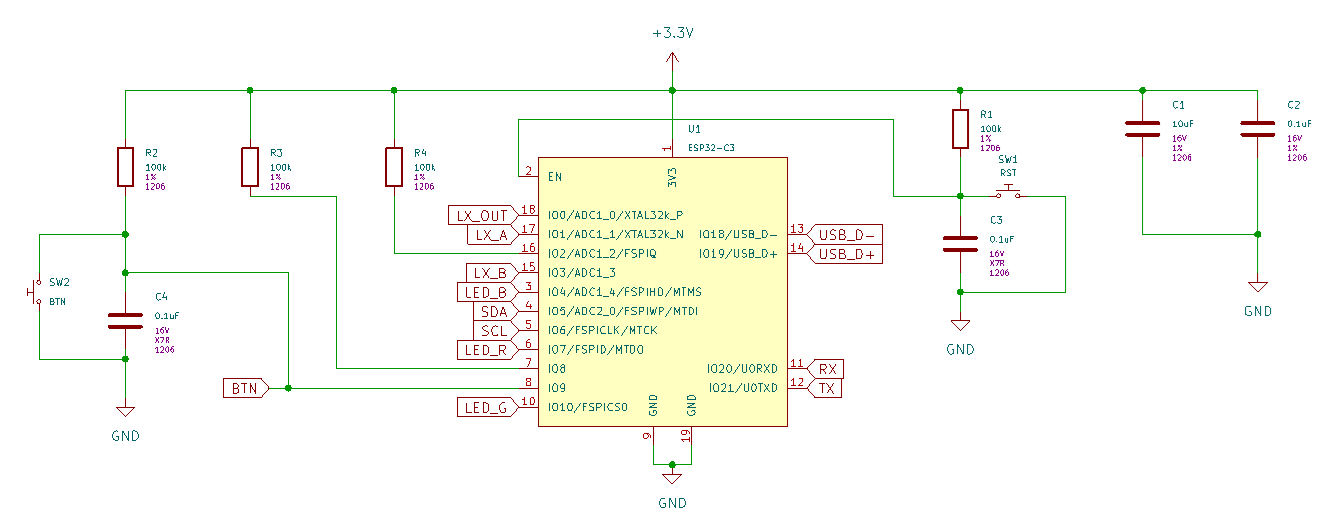
\includegraphics[width=1\textwidth]{Imgs/blok1.png}
    \caption{Blokovna shema razvojne plošče}
    \label{fig:blok_shema}
\end{figure}

\section{Sestavni elementi}
\begin{itemize}
    \item Mikrokrmilnik: ESP32-C3-WROOM-02 \\
    Povezava do podatkovnega lista: \url{https://eu.mouser.com/datasheet/2/891/Espressif_Systems_04082021_ESP32_C3_WROOM_02-2295851.pdf} \\
    Mikrokrmilnik predstavlja osrednji element razvojne plošče, saj upravlja delovanje vseh ostalih komponent in izvaja obdelavo podatkov. Gre za zmogljivo enoto s široko možnostjo uporabe – od osnovnega nadzora senzorjev do naprednejših aplikacij. Poleg klasičnih funkcij je podprta tudi brezžična komunikacija prek tehnologij Wi-Fi in BLE.

    \item USB-C priključek – Molex216990-001  \\
    Povezava do podatkovnega lista: \url{https://www.molex.com/content/dam/molex/molex-dot-com/products/automated/en-us/salesdrawingpdf/216/216990/2169900001_sd.pdf} \\
    Omogoča enostavno povezavo z računalnikom za napajanje in prenos podatkov.
    \begin{figure}[H]
        \centering
        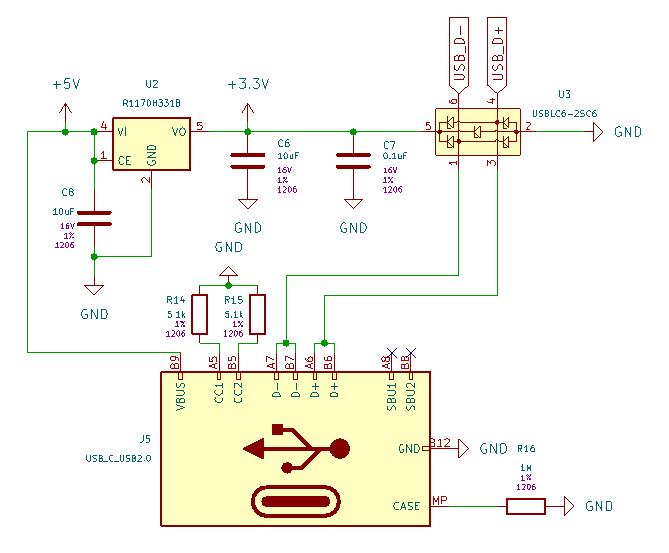
\includegraphics[width=0.8\linewidth]{Imgs/blok2.png}
        \caption{Blokovna shema USB-C priključka, ESD-ja in regulatorja napetosti}
        
    \end{figure}

    \item ESD(Electrostatic discharge) protection - USBLC6-2SC6 \\
    Povezava do podatkovnega lista: \url{https://eu.mouser.com/datasheet/2/389/usblc6_2-1852789.pdf} \\
    Gre za element, ki ščiti vezje pred škodljivimi vplivi elektrostatičnih razelektritev. Zaradi zelo nizke lastne kapacitivnosti ne vpliva na delovanje hitrih podatkovnih linij. Hkrati učinkovito omejuje tokovne sunke, ki bi lahko poškodovali občutljive komponente.

    \item LDO(Low dropout regulator) - R1170H331B-T1-FE \\
    Povezava do podatkovnega lista: \url{https://eu.mouser.com/datasheet/2/294/r1170_ea-3219814.pdf} \\
    Nizko-izgubni linearni regulator napetosti skrbi za pretvorbo vhodnih 5 V v stabilno delovno napetost 3,3 V. Izdelan je v CMOS tehnologiji, kar zagotavlja visoko energijsko učinkovitost, saj porabi energijo predvsem med preklopi stikalnih tranzistorjev.
    
    \item RGB LED - HV-5RGB60 \\
    Povezava do podatkovnega lista: \url{https://eu.mouser.com/datasheet/2/180/HV_5RGBXX_5mm_Full_Color_Series-1489147.pdf} \\
    Večbarvna LED dioda, z ločenimi rdečimi, zelenimi in modrimi elementi, omogoča generiranje različnih barv s pomočjo ustreznega krmiljenja PWM signalov. Standardni tok skozi diodo znaša 25 mA, maksimalni dovoljen impulz pa doseže do 100 mA za zelo kratek čas.
    
    \item Tipka - PTS645SM50SMTR92 LFS  \\
    Povezava do podatkovnega lista: \url{https://www.ckswitches.com/media/1471/pts645.pdf}  \\   
    Gre za SMD momentno stikalo, namenjeno ponastavitvi delovanja mikrokrmilnika med razvojem ali testiranjem programa. Zagotavlja mehansko zanesljivost do 100.000 pritiskov,  deluje do toka 50 mA pri napetosti 12 V.
    
    \item Senzor svetlobe - TEPT5700 \\
    Povezava do podatkovnega lista: \url{https://www.vishay.com/docs/81321/tept5700.pdf} \\    
    To je NPN fototranzistor, občutljiv na svetlobo v spektru vidne svetlobe. Z naraščanjem jakosti svetlobe se povečuje tok skozi senzor, kar omogoča zaznavo ambientne svetlobe.
    \begin{figure}[H]
        \centering
        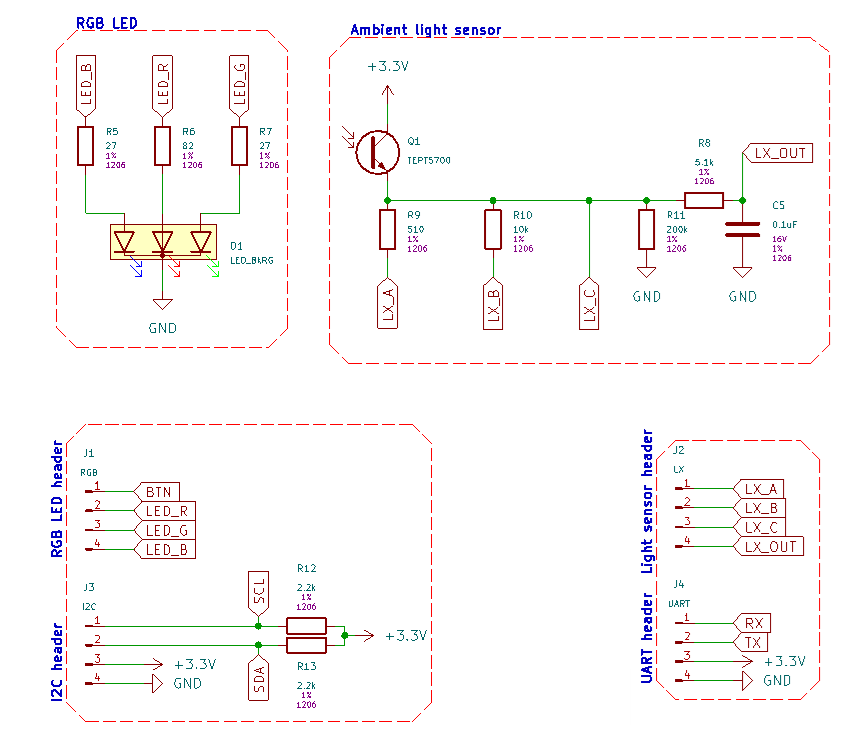
\includegraphics[width=0.9\linewidth]{Imgs/blok3.png}
        \caption{Blokovna shema ostalih modulov}
        \label{fig:enter-label}
    \end{figure}
\end{itemize}

\section{Razporeditev elementov}

\begin{figure}[H]
\centering
\begin{subfigure}{.4\textwidth}
  \centering
  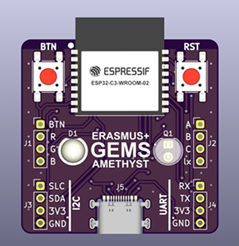
\includegraphics[width=.9\linewidth]{Imgs/board1.png}
\end{subfigure}
\begin{subfigure}{.4\textwidth}
  \centering
  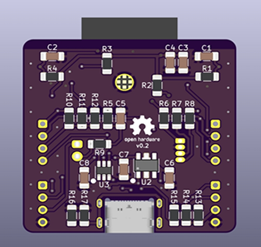
\includegraphics[width=.9\linewidth]{Imgs/board2.png}
\end{subfigure}
\caption{Razvojna plošča}
\end{figure}

\section{Tehnične specifikacije}
\begin{table}[H]
\centering
\caption{Tehnične specifikacije razvojne plošče GEMS Amethyst}
\begin{tabular}{|l|p{10cm}|}
\hline
\textbf{Parameter} & \textbf{Vrednost} \\
\hline
Mikrokrmilnik & ESP32-C3-WROOM-02 (RISC-V 32-bitni, 160 MHz, Wi-Fi + BLE 5.0) \\
\hline
Vhodna napetost (USB) & 5 V prek USB-C \\
\hline
Obratovalna napetost & 3.3 V (regulirana) \\
\hline
Maksimalni izhodni tok & 300 mA \\
\hline
Tipična poraba toka & $\sim$80 mA aktivno (Wi-Fi vklopljen), <10 µA v globokem spanju \\
\hline
Brezžični vmesniki & Wi-Fi 802.11 b/g/n (2.4 GHz), Bluetooth LE 5.0 \\
\hline
USB vmesnik & USB 2.0 Full-Speed (z ESD zaščito) \\
\hline
ESD zaščita & $\pm$15 kV (zrak), $\pm$8 kV (kontakt) \\
\hline
Senzor svetlobe & TEPT5700 – največja občutljivost pri $\sim$570 nm (vidna svetloba) \\
\hline
Podprti vmesniki & UART, SPI, I\textsuperscript{2}C, PWM, ADC (12-bitni), GPIO \\
\hline
Dimenzije plošče & 45mm x 40mm \\
\hline
Obratovalna temperatura & -40~$^\circ$C do +85~$^\circ$C \\
\hline
\end{tabular}
\label{tab:amethyst_spec_sl}
\end{table}



\section{Fizične povezave in izdelava}
Plošča uporablja dvoplastni PCB, ki vsebuje več plasti bakra. Te plasti omogočajo povezavo med različnimi elektronskimi komponentami na plošči. V našem primeru imamo bakrene plasti na obeh straneh plošče. Glavna funkcija bakrenih plasti je zagotavljanje poti za električne signale med različnimi komponentami na PCB-ju. Te poti so oblikovane kot sledilne poti, ki so izrezane iz bakrene plasti. Na zunanji plasti bakra se oblikujejo plastični odseki, ki so izolirani od zunanjih plasti ter med seboj s plastmi epoksidne smole. Proces izdelave PCB-ja se začne z načrtovanjem vezja v elektronskem CAD programu (KiCad), kjer se določijo postavitve komponent, sledi bakra in lokacije lukenj za montažo. Nato se izdela fotomaska, ki temelji na načrtovanem vezju in vsebuje informacije o sledi poti ter lokacijah lukenj za komponente. Substrat PCB-ja se pripravi z nanašanjem tankih plasti bakra (sledi poti) na obeh straneh. Sledi se ustvarijo s pomočjo fotomaske, ki ščiti bakreni sloj med izpostavljanjem izbranih delov bakra UV svetlobi za utrjevanje sledi. Nezaščiteni deli bakra se nato jedkajo, da se ustvarijo sledi za električne povezave. Po tem se izvrta luknje za montažo komponent. Na koncu sledi še namestitev komponent na PCB in pritrditev komponent z lotanjem. Pri oblikovanju PCB-ja je pomembno upoštevati širino in debelino sledilnih poti (traces) ter razporeditev bakrenih plasti, da se zagotovi ustrezna električna zmogljivost in zanesljivost vezja. Poleg tega se bakrene plasti uporabljajo tudi za izdelavo površinskih kontaktnih točk, ki omogočajo pritrditev in lotanje elektronskih komponent na PCB-ju.

Pri spajkanju elementov, kot so upori, pa je potrebna pazljivost.

\textbf{Navodilo za spajkanje:}
\begin{itemize}
    \item Najprej pripravimo razvojno ploščico in komponente, ki jih želimo lotati. 
    \item Potem namažemo ploščico s flux-om. 
    \item Nastavimo spajkalnik na približno 350 °C. 
    \item Nanesemo majhno količino spajke na eni strani kontakta, drugo stran lotamo potem. 
    \item Položimo komponente na kontakte ter s spajkalnikom zgrejemo spajke in tako ustvarimo povezave. 
    \item Ko smo končali z lotanjem vseh uporov na eni strani, potem zalotamo še drugo stran. 
    \item Na koncu preverimo vse lotane povezave in se prepričamo, da ni hladnih spojev ali kratkih stikov.
\end{itemize}

\textbf{Primer spremembe povezave:} Odklop LED in priklop zunanje LED prek pina LED\_R z uporom.

\chapter{Delovanje razvojne plošče}
    \section{Glavne funkcije}
Razvojna plošča vključuje RGB LED, gumb, senzor osvetlitve z možnostjo zamenjave pull-down uporov za zmanjšanje tolerance senzorja, UART, I2C, WiFi, BLE in serijsko komunikacijo. Primerna je za IoT projekte in projekte, ki temeljijo na merjenju in upravljanju glede na ambientalno svetlobo.

\section{Programiranje in okolje}
Programiranje te razvojne plošče poteka preko Arduino IDE, ki je dostopen na \url{https://www.arduino.cc/en/software/}. Poleg tega je treba namestiti še paket plošč esp32.

\subsection{Namestitev paketa esp32}
Za namestitev paketa esp32 pojdite na Tools→Board→Board Manager ali kliknite ikono na levi strani. Poiščite "esp32 by Espressif Systems" in kliknite Install. Če je bilo uspešno nameščeno, se bo pod Tools→Board pojavila možnost esp32, znotraj katere so vse esp32 plošče, vključno z ESP32C3 Dev Module, ki je naša plošča.

\begin{figure}[H]
    \centering
    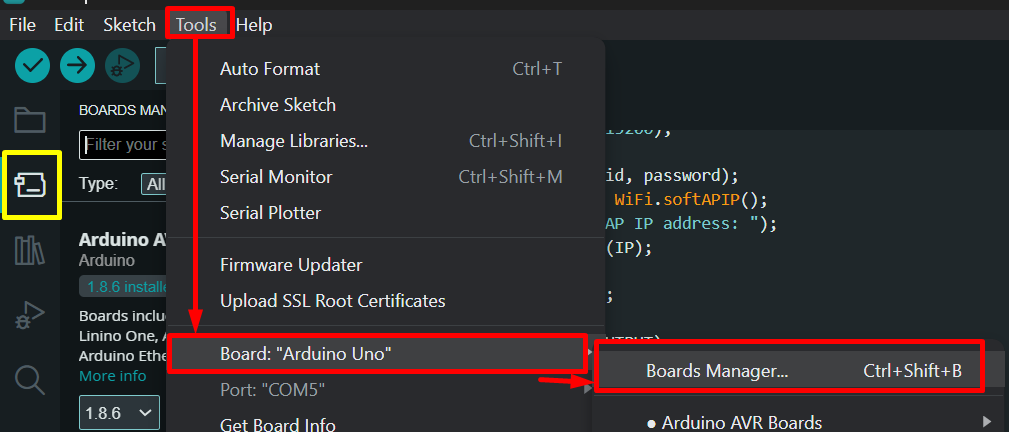
\includegraphics[width=0.9\linewidth]{Imgs/boardsetup1.png}
    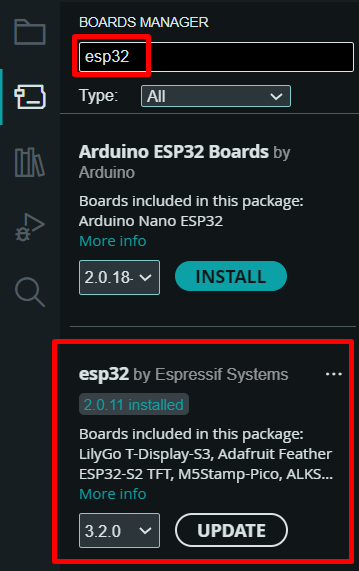
\includegraphics[width=0.5\linewidth]{Imgs/boardsetup2.png}
    \caption{Namestitev paketa esp32}
    \label{fig:enter-label}
\end{figure}

\subsection{Postopek nalaganja programa}
Za nalaganje programa na ploščo jo priključite preko USB-ja, preverite da so nastavitve plošče ustrezne (spodaj navedene), in kliknite Upload. Ko piše "done uploading", lahko ploščo odklopite.
Board settings: 
\begin{enumerate}
    \item Board: ESP32C3 Dev Module
    \item Port: ustrezen COM port
    \item USB CDC On Boot: Enabled 
    \item CPU Frequency: 80MHz
\end{enumerate}

\section{Pomembni pini}
\begin{enumerate}
    \item Gumb: 9
    \item Rdeča LED: 7
    \item Zelena LED: 10
    \item Modra LED: 4
    \item LX\_A: 1
    \item LX\_B: 3
    \item LX\_OUT: 0
    \item SDA: 5
    \item SCL: 6
    \item RX: 20
    \item TX: 21
\end{enumerate}

\section{Uporaba light sensorja}
Z zamenjavo stanj pinov LX\_A in LX\_B na HIGH ali LOW(to lahko naredite tudi ročno s spreminjanjem uporov prek jumperjev) lahko spreminjate občutljivost svetlobnega senzorja. Spodaj je primer kode, kjer lahko z izbiro mode 1, 2 ali 3 spreminjate območje izmerjene izhodne napetosti.

\begin{lstlisting}[language=Arduino]
#define LX_A 1
#define LX_B 3
#define LX_OUT 0

void setup() {
  Serial.begin(115200);

  pinMode(LX_A, OUTPUT);
  pinMode(LX_B, OUTPUT);
  pinMode(LX_OUT, INPUT);

  Serial.println("Select mode:");
  Serial.println("Mode 1");
  Serial.println("Mode 2");
  Serial.println("Mode 3");
}

void loop() {
  if (Serial.available() > 0) {
    char c = Serial.read();

    switch (c) {
      case '1':  // Mode 1
        digitalWrite(LX_A, LOW);  
        digitalWrite(LX_B, LOW);  
        Serial.println("Mode set to 1");
        break;
      case '2':  // Mode 2
        digitalWrite(LX_A, LOW); 
        digitalWrite(LX_B, HIGH);
        Serial.println("Mode set to 2");
        break;
      case '3':  // Mode 3
        digitalWrite(LX_A, HIGH);  
        digitalWrite(LX_B, LOW); 
        Serial.println("Mode set to 3");
        break;
    }
  }

  int output = analogRead(LX_OUT);

  Serial.println(output);

  delay(100);
}
\end{lstlisting}

\section{Primeri funkcije}
\subsection{RGB LED}
Povezava do knjižnice: \url{https://docs.arduino.cc/language-reference/en/functions/digital-io/digitalwrite/}
\begin{lstlisting}[language=Arduino]  
#define LED_R 7
#define LED_G 10
#define LED_B 4

void setup() {
  pinMode(LED_R, OUTPUT);
  pinMode(LED_G, OUTPUT);
  pinMode(LED_B, OUTPUT);
}

void loop() {
  analogWrite(LED_R, 255); // red
  analogWrite(LED_G, 0);
  analogWrite(LED_B, 0);
  delay(1000);

  analogWrite(LED_R, 0);
  analogWrite(LED_G, 255); // green
  analogWrite(LED_B, 0);
  delay(1000);

  analogWrite(LED_R, 0);
  analogWrite(LED_G, 0);
  analogWrite(LED_B, 255); // blue
  delay(1000);
}
\end{lstlisting}

\subsection{Gumb}
Povezava do knjižnice: \url{https://docs.arduino.cc/language-reference/en/functions/digital-io/digitalread/}
\begin{lstlisting}[language=Arduino]  
#define BTN 9
#define LED_R 7

void setup() {
  pinMode(BTN, INPUT_PULLUP);
  pinMode(LED_R, OUTPUT);
}

void loop() {
  if (digitalRead(BTN) == LOW) {
    digitalWrite(LED_R, HIGH); // button pressed
  } else {
    digitalWrite(LED_R, LOW);
  }
}    
\end{lstlisting}

\subsection{Light sensor}
Povezava do knjižnice: \url{https://docs.arduino.cc/language-reference/en/functions/analog-io/analogRead/}
\begin{lstlisting}[language=Arduino]  
#define LX_A 1
#define LX_B 3
#define LX_OUT 0

void setup() {
  Serial.begin(115200);
  delay(300);
}

void loop() {
  int lightLevel = lx(1);
  Serial.print("Light Level: ");
  Serial.println(lightLevel);
  delay(500);
}

int lx(int mode) {
  switch (mode) {
    case 0:
      pinMode(LX_A, INPUT);
      pinMode(LX_B, INPUT);
      break;
    case 1:
      pinMode(LX_A, INPUT);
      pinMode(LX_B, OUTPUT);
      digitalWrite(LX_B, LOW);
      break;
    case 2:
      pinMode(LX_A, OUTPUT);
      digitalWrite(LX_A, LOW);
      pinMode(LX_B, INPUT);
      break;
    default:
      pinMode(LX_A, INPUT);
      pinMode(LX_B, INPUT);
  }

  return analogRead(LX_OUT);
}
\end{lstlisting}

\subsection{Serial komunikacija}
Povezava do knjižnice: \url{https://www.arduino.cc/reference/en/language/functions/communication/serial/}
\begin{lstlisting}[language=Arduino]  
void setup() {
  Serial.begin(115200);
  delay(1000);
  Serial.println("Serial is working!");
}

void loop() {
  if (Serial.available()) {
    String input = Serial.readStringUntil('\n');
    Serial.print("You said: ");
    Serial.println(input);
  }
}
\end{lstlisting}

\subsection{Wi-fi}
Povezava do knjižnice: \url{https://docs.arduino.cc/libraries/wifi/}
\begin{lstlisting}[language=Arduino]  
#include <WiFi.h>

const char* ssid = "SSID";
const char* password = "PASSWD";
WiFiServer server(80);

void setup() {
  Serial.begin(115200);
  delay(1000);

  Serial.print("Connecting to ");
  Serial.println(ssid);
  WiFi.begin(ssid, password);

  while (WiFi.status() != WL_CONNECTED) {
    delay(500);
    Serial.print(".");
  }

  Serial.println("");
  Serial.println("WiFi connected.");
  Serial.print("IP address: ");
  Serial.println(WiFi.localIP());

  server.begin();
}

void loop() {
  WiFiClient client = server.available(); 

  if (client) {
    Serial.println("New Client.");
    String request = client.readStringUntil('\r');
    Serial.println(request);
    client.flush();

    client.println("HTTP/1.1 200 OK");
    client.println("Content-type:text/html");
    client.println();
    client.println("<!DOCTYPE html><html><body><h1>Mehatronika</h1></body></html>");
    client.println();
    client.stop();
    Serial.println("Client disconnected.");
  }
}
\end{lstlisting}

\subsection{Bluetooth}
Povezava do knjižnice: \url{https://github.com/nkolban/ESP32_BLE_Arduino}
\begin{lstlisting}[language=Arduino]  
#include <BLEDevice.h>
#include <BLEUtils.h>
#include <BLEServer.h>

#define SERVICE_UUID        "4fafc201-1fb5-459e-8fcc-c5c9c331914b"
#define CHARACTERISTIC_UUID "beb5483e-36e1-4688-b7f5-ea07361b26a8"

void setup() {
  Serial.begin(115200);
  Serial.println("Starting BLE work!");

  BLEDevice::init("Long name works now");
  BLEServer *pServer = BLEDevice::createServer();
  BLEService *pService = pServer->createService(SERVICE_UUID);
  BLECharacteristic *pCharacteristic = pService->createCharacteristic(
                                         CHARACTERISTIC_UUID,
                                         BLECharacteristic::PROPERTY_READ |
                                         BLECharacteristic::PROPERTY_WRITE
                                       );

  pCharacteristic->setValue("Hello World says Neil");
  pService->start();
  BLEAdvertising *pAdvertising = BLEDevice::getAdvertising();
  pAdvertising->addServiceUUID(SERVICE_UUID);
  pAdvertising->setScanResponse(true);
  pAdvertising->setMinPreferred(0x06);
  pAdvertising->setMinPreferred(0x12);
  BLEDevice::startAdvertising();
  Serial.println("Characteristic defined! Now you can read it in your phone!");
}
\end{lstlisting}

\subsection{I2C}
Povezava do knjižnice: \url{https://www.arduino.cc/en/Reference/Wire}
\begin{lstlisting}[language=Arduino]  
#include <Wire.h>
#define SDA 5
#define SCL 6

void setup() {
  Wire.begin(SDA, SCL);
  Serial.begin(115200);
  delay(1000);
  Serial.println("I2C Scanner starting...");

  for (uint8_t address = 1; address < 127; ++address) {
    Wire.beginTransmission(address);
    if (Wire.endTransmission() == 0) {
      Serial.print("I2C device found at address 0x");
      Serial.println(address, HEX);
    }
    delay(5);
  }

  Serial.println("Scan complete.");
}
\end{lstlisting}

\subsection{UART}
Povezava do knjižnice: \url{https://docs.arduino.cc/learn/communication/uart/}
\begin{lstlisting}[language=Arduino]
#define RX 20
#define TX 21

void setup() {
  Serial.begin(115200);               // USB Serial Monitor
  Serial1.begin(9600, SERIAL_8N1, RX, TX); // UART Serial
  Serial.println("UART echo demo started...");
}

void loop() {
  if (Serial1.available()) {
    char c = Serial1.read();     // Read from UART
    Serial1.write(c);            // Echo back to UART
    Serial.print("Received: ");
    Serial.println(c);           // Also print to USB serial for debugging
  }
}

\end{lstlisting}





\end{document}

\end{document}
